I have worked out the part on stiffness determination for a very large extend. Those parts are marked in blue. 


\textbf{To discuss}
\begin{itemize}
    \item Coupling rotation and elongation. Based on the current data an easy interaction can be found, however we should discuss if this is a valid assumption.
    \item Adapted planning
    \item Next steps
    \item How to visualize c++ results in matlab? I forgot
    \item Nog recentere versie van de code, up to date zip.
    
\end{itemize}


I also started projecting backbone curve to $l_1$ and $l_2$ this is shown in Figure \ref{fig:progress}. I have not started on a numerical integration for finding $V_q$.


\begin{figure}[H]
    \centering
    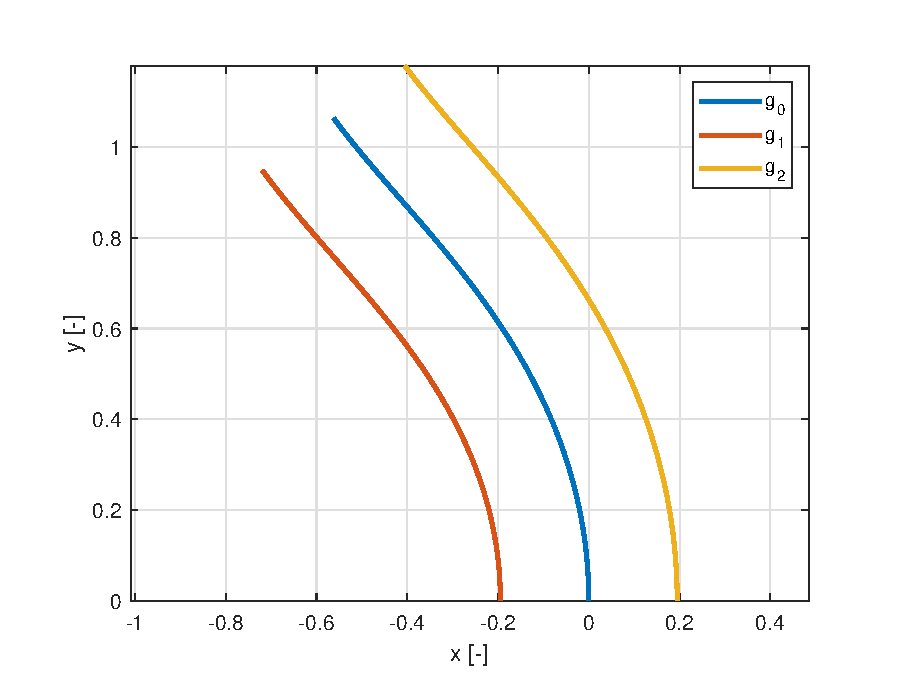
\includegraphics[width = 0.5\textwidth]{Figures/ProgresFigures/g0g1g2.eps}
    \caption{Backbone curve ($g_0$) and projection to $g_1$ and $g_2$}
    \label{fig:progress} 
\end{figure}

By multiplying $g_i$ with initial length $L_0$ lengths $L_1$ and $L_2$ can be found, shown in Figure (\ref{fig:progress2}).

\begin{figure}[H]
    \centering
    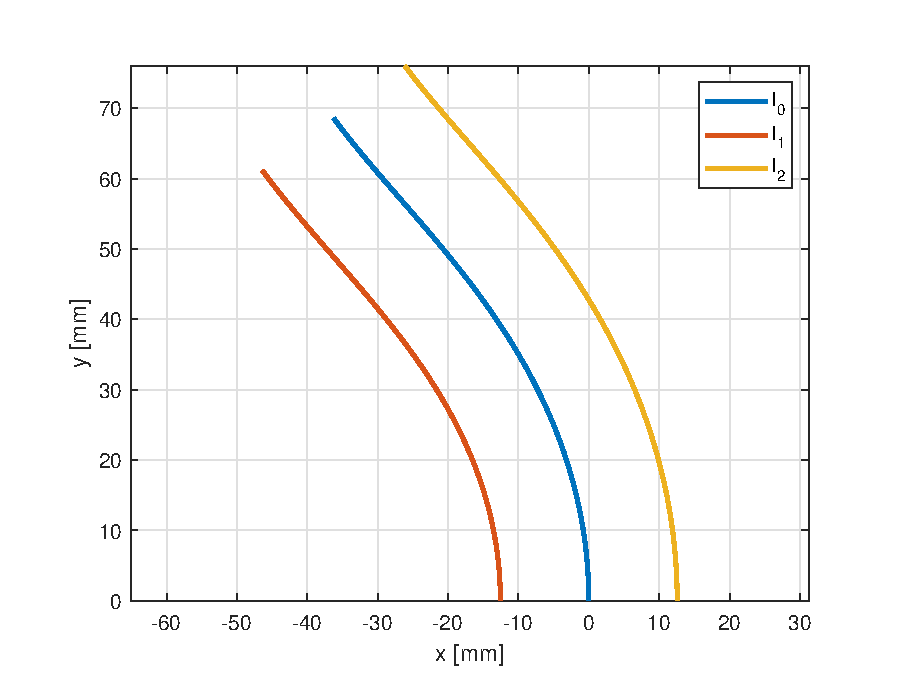
\includegraphics[width = 0.5\textwidth]{Figures/ProgresFigures/l0l1l2.eps}
    \caption{Backbone curve and projection to $g_1$ and $g_2$}
    \label{fig:progress2} 
\end{figure}